\documentclass{article}

\usepackage{listings} % for including MATLAB code
\usepackage{graphicx} % for including images
\usepackage{amsmath}

\title{80846 - Report - 3rd}
\author{GU JUN, 6132230056-4}
\date{\today}

\begin{document}

\maketitle

\section*{Introduction}

The following content will be organized in the following way: First is about passivity-based task-space controller, then is a computed torque controller. 
\\
Each part will be organized by Problem Statement, Simulink model, Source codes for RobotDynamics and controller blocks, Simulation results, and Explanation.

\section*{\centering \Huge Passivity-based task-space controller}

\section*{Problem Statement}

According to the class, we are required to complete the \\
1. Jacobian matrix \\
2. A block for forward kinematics: \\


% model of the system
\section{Simulink Model}
See the Figure \ref{fig:model_task_model} below. The whole system includes two subsystems: RobotDynamics and Controller.
\begin{figure}[ht]
    \centering
    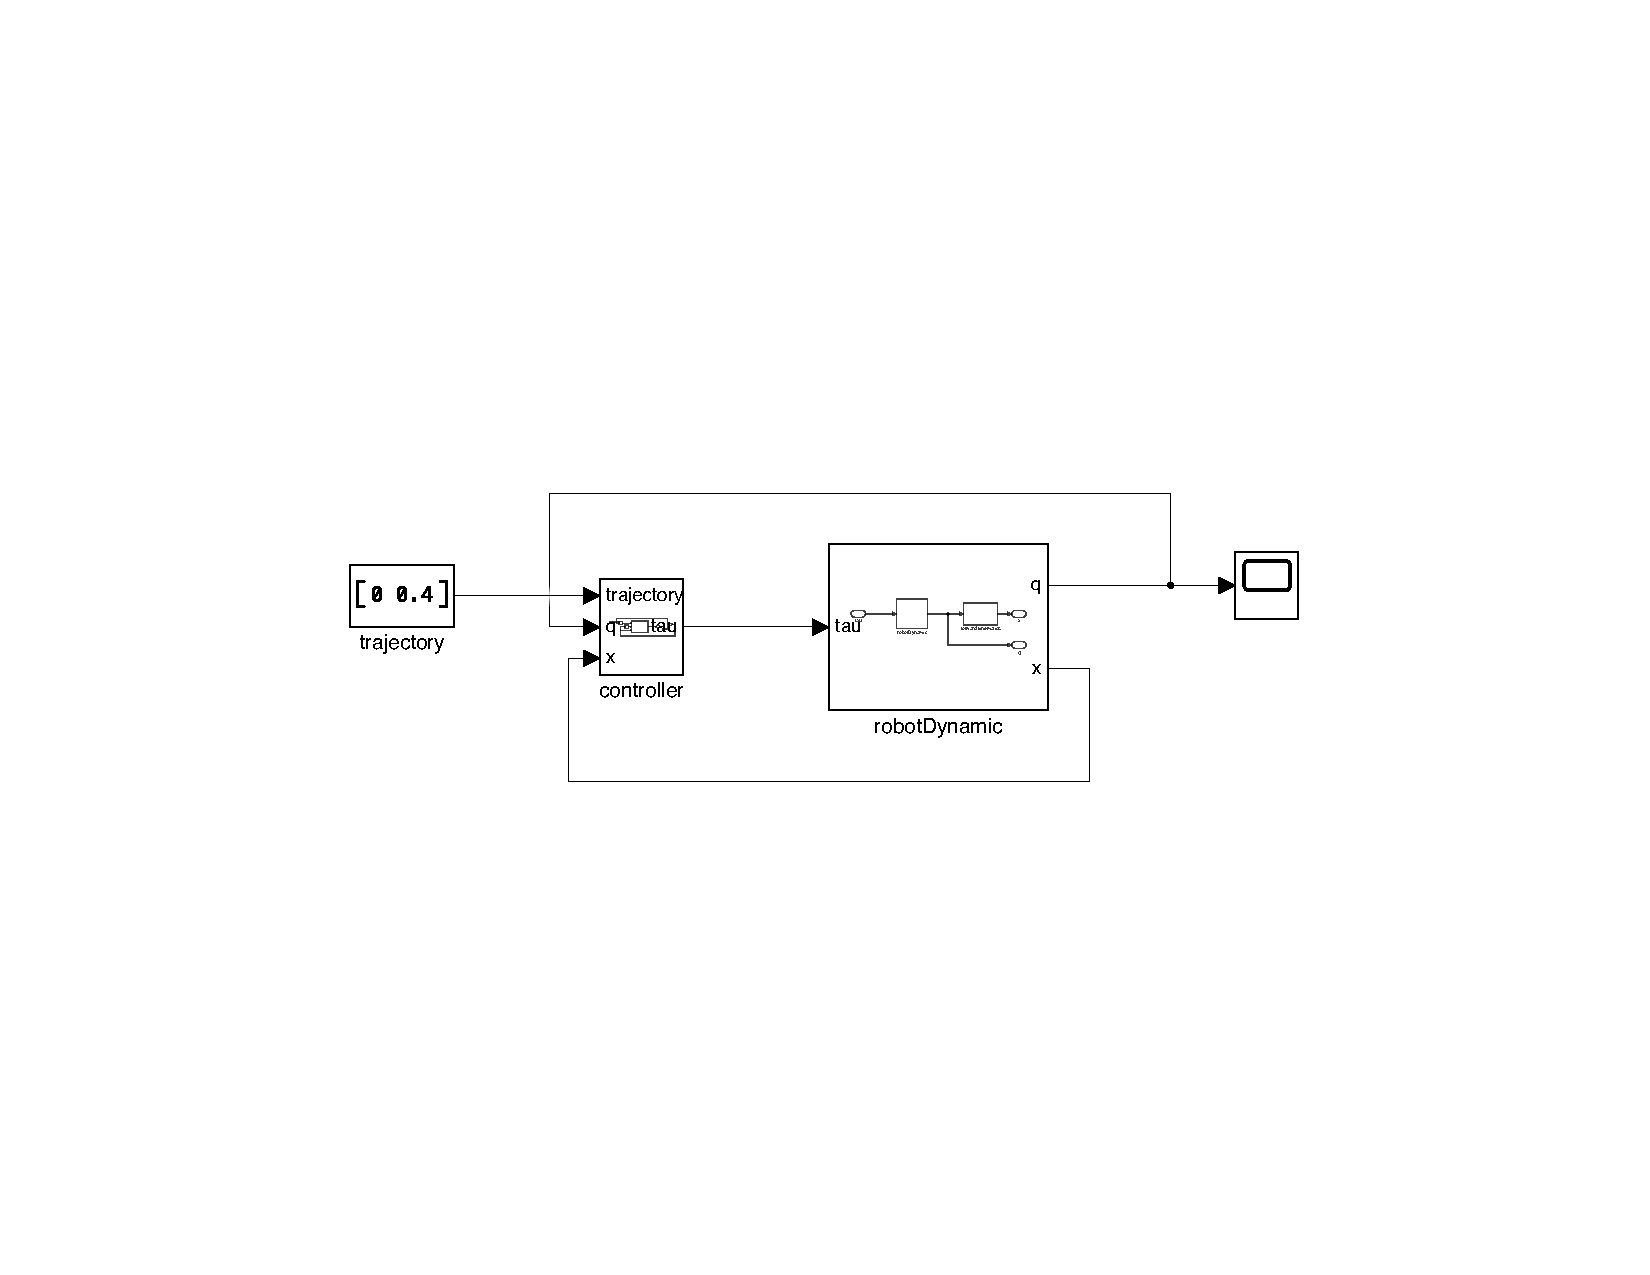
\includegraphics[width=0.9\textwidth]{figures/model_task_space.pdf}
    \caption{Simulink Model of the whole system}
    \label{fig:model_task_model}
\end{figure}

% formulas and source codes
\section{Formulas and Source Codes}
This part includes the formulas and source codes for the controller with the Jacobian matrix and forward kinematics blocks.
\subsection*{Jacobian matrix}
The Jacobian matrix is calculated by the following formula:\\
\[
J = \begin{bmatrix}
    \frac{\partial x}{\partial \theta_1} & \frac{\partial x}{\partial \theta_2} \\
    \frac{\partial y}{\partial \theta_1} & \frac{\partial y}{\partial \theta_2}
\end{bmatrix}
\]
\[
= \begin{bmatrix}
    -l_1 \sin(\theta_1) - l_2 \sin(\theta_1 + \theta_2) & -l_2 \sin(\theta_1 + \theta_2) \\
    l_1 \cos(\theta_1) + l_2 \cos(\theta_1 + \theta_2) & l_2 \cos(\theta_1 + \theta_2)
\end{bmatrix}
\]

    

The source code is shown below:
\begin{lstlisting}[language=Matlab, basicstyle=\small\ttfamily]

function tau = controller(error, derror, q)

lg1 = 0.2;
lg2 = 0.2;

kp = [800, 0;
       0, 800];


kd = [1, 0;
        0, 1];

jacobian = [-lg1 * sin(q(1)) - lg2 * sin(q(1) + q(2)), -lg2 * sin(q(1) + q(2));
    lg1 * cos(q(1)) + lg2 * cos(q(1) + q(2)), lg2 * cos(q(1) + q(2))];


tau = kp * transpose(jacobian) * error - kd * derror;
end

\end{lstlisting}

\subsection*{Forward Kinematics}

Forward Kinematics is calculated by\\

\begin{equation}
    x = l_1 cos(\theta_1) + l_2 cos(\theta_1 + \theta_2)
\end{equation}
\begin{equation}
    y = l_1 sin(\theta_1) + l_2 sin(\theta_1 + \theta_2)
\end{equation}


The source code is shown below:
\begin{lstlisting}[language=Matlab,  basicstyle=\small\ttfamily]

function x = kinematics(q)

lg1 = 0.2;
lg2 = 0.2;
x = [0;
    0];
x(1) = lg1 * cos(q(1)) + lg2 * cos(q(1) + q(2));
x(2) = lg1 * sin(q(1)) + lg2 * sin(q(1) + q(2));

end

\end{lstlisting}

\section{Simulation Results}

As a result, I got the following Figure \ref{fig:result_task_space_plot}. \\
\begin{figure}[ht]
    \centering
    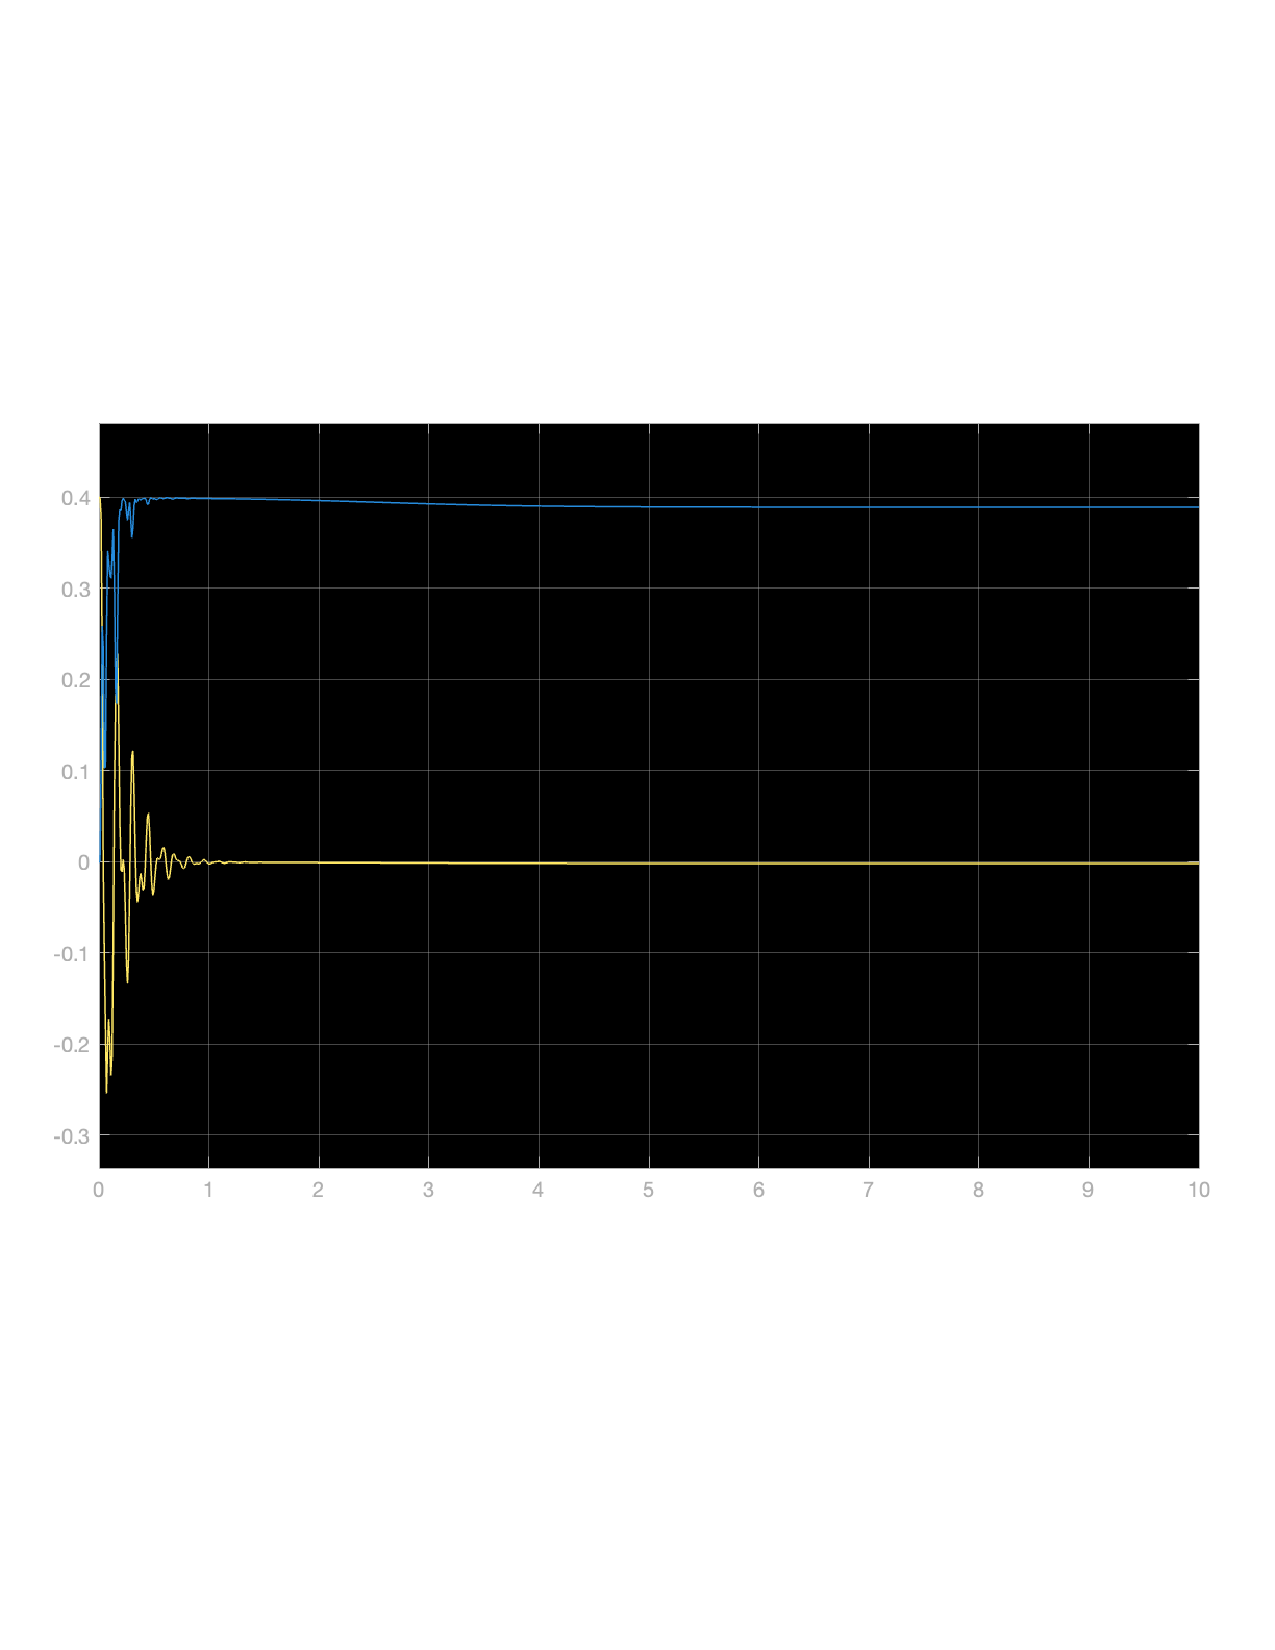
\includegraphics[width=0.8\textwidth]{figures/result_task_space.pdf}
    \caption{Result Plot with a target of (0, 0.4).}
    \label{fig:result_task_space_plot}
\end{figure}



\setcounter{section}{0}


\newpage

\section*{\centering \Huge Computed torque controller}

\section*{Problem Statement}

According to the class, we are required to complete a controller that can track a torque function $q_d(t)$. I use the $sin$ function with $0.5 \pi$ shift on $y$.

% model of the system
\section{Simulink Model}
See the Figure \ref{fig:model_computed} below.
\begin{figure}[ht]
    \centering
    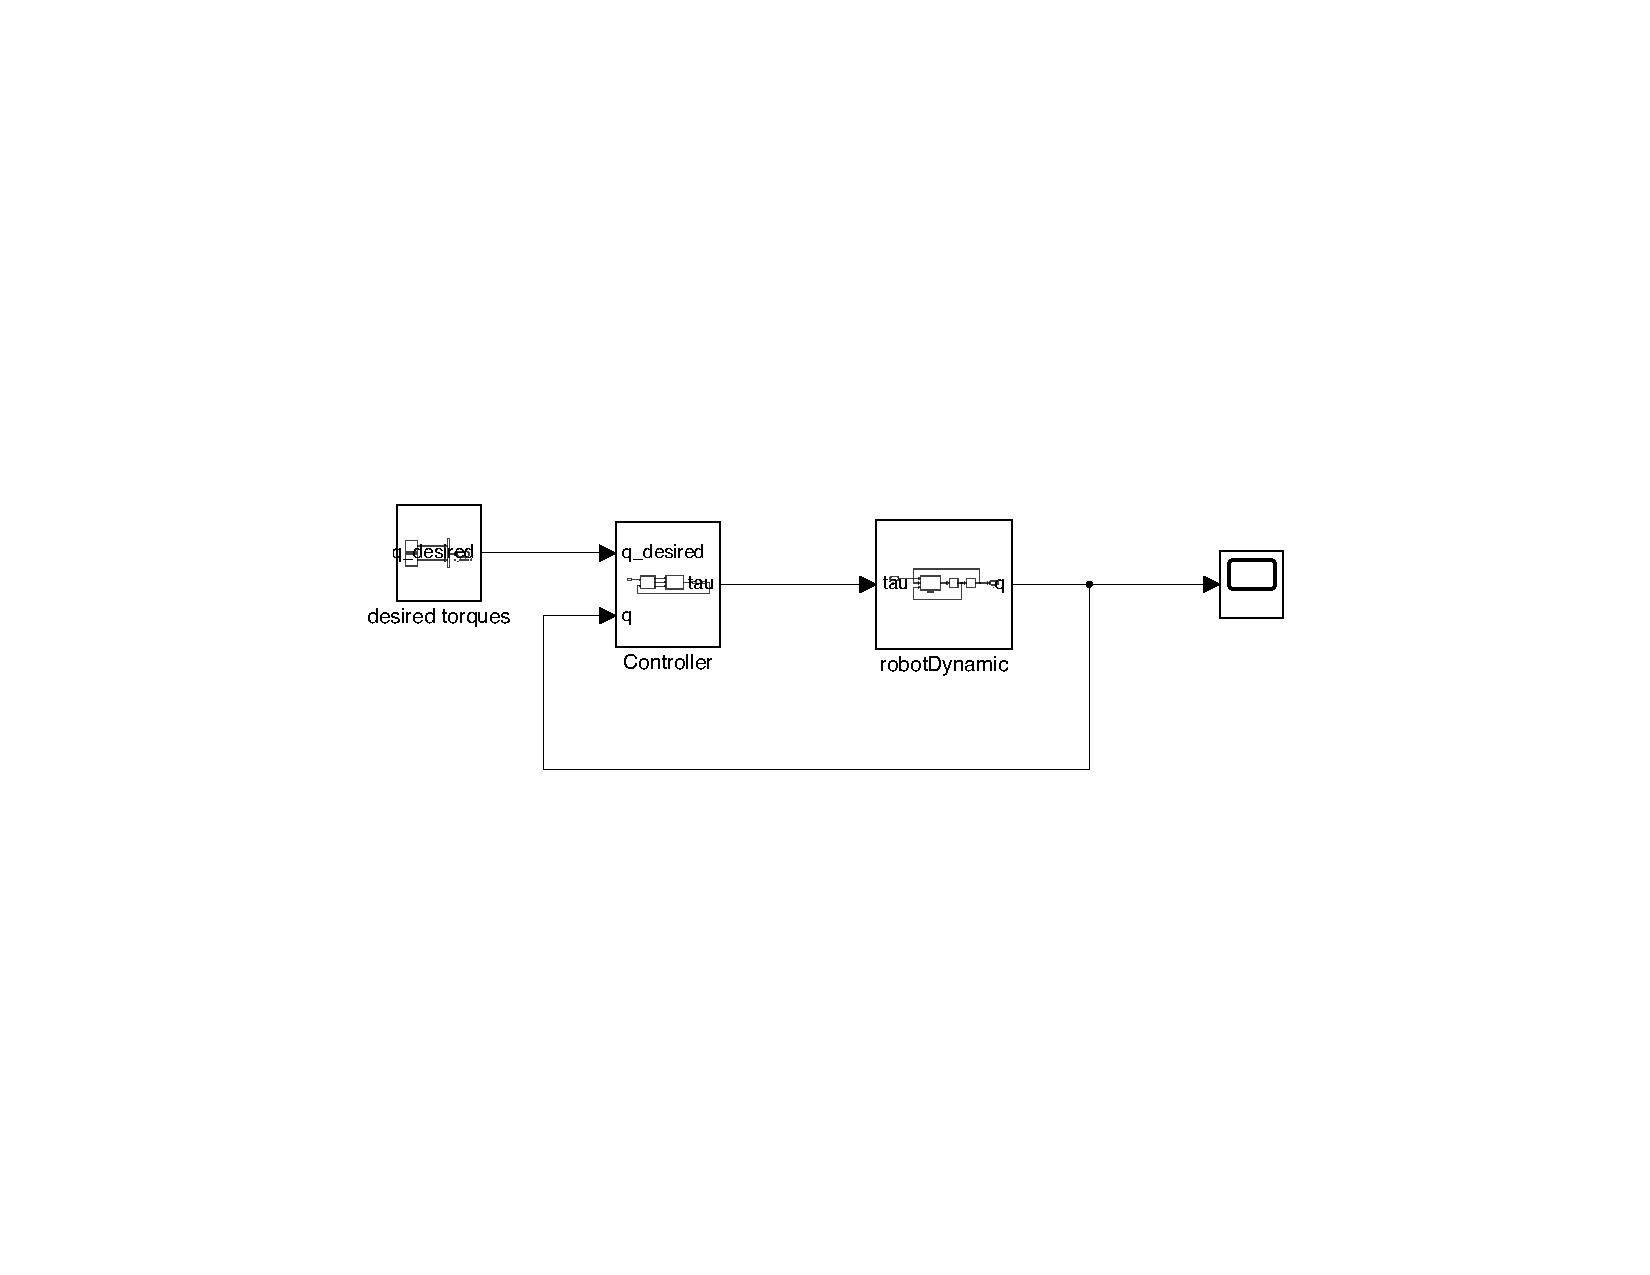
\includegraphics[width=0.9\textwidth]{figures/model_computed.pdf}
    \caption{Simulink Model of the system for the Computed torque controller}
    \label{fig:model_computed}
\end{figure}

% formulas and source codes
\section{Formulas and Source Codes}
This part includes the formulas and source codes for the inverse dynamics
\subsection*{Inverse Dynamics}
According to the formula below, we need to calculate the $\tau_d$\\
    \begin{equation}
        \tau=\tau_d+k_p(q_d-q)+k_v(\dot{q}_d-\dot{q})
    \end{equation}
To calculate $\tau_d$, I use inverse dynamics.\\ 
\begin{equation}
    \tau_d = M \Ddot{q_d} + V \dot{q_d} + G
\end{equation}
Where $M$, $V$, $G$ have been mentioned in the past lectures.\\
The source code is shown below:
\begin{lstlisting}[language=Matlab, basicstyle=\small\ttfamily]


I1 = 0.05;
m1 = 1.5;
lg1 = 0.2;
lr1 = lg1 / 2;

I2 = 0.01;
m2 = 0.5;
lg2 = 0.2;
lr2 = lg2 / 2;

g = 9.8;

M = [m1 * lr1^2 + I1 + m2 * lg1^2, m2 * lg1 * lr2 * cos(q_desired(2));
        m2 * lg1 * lr2 * cos(q_desired(2)), m2 * lr2^2 + I2];

V = [-m2 * lg1 * lr2 * qd_desired(2)^2 * sin(q_desired(2));
    m2 * lg1 * lr2 * qd_desired(1)^2 * sin(q_desired(2))];

G = [m1 * g * lr1 * cos(q_desired(1)) + m2 * g * lg1 * cos(q_desired(1));
    m2 * g * lr2 * cos(q_desired(1) + q_desired(2));];

tau_d = M * qdd_desired + V + G;

    
\end{lstlisting}

\subsection*{Controller}
For the controller, there is just a little change.\\

The source code is shown below:\\

\begin{lstlisting}[language=Matlab, basicstyle=\small\ttfamily]
    
\end{lstlisting}

\section{Simulation Results}

After some tuning of the gains, I got the following Figure \ref{fig:result_computed_plot}. \\
\begin{figure}[ht]
    \centering
    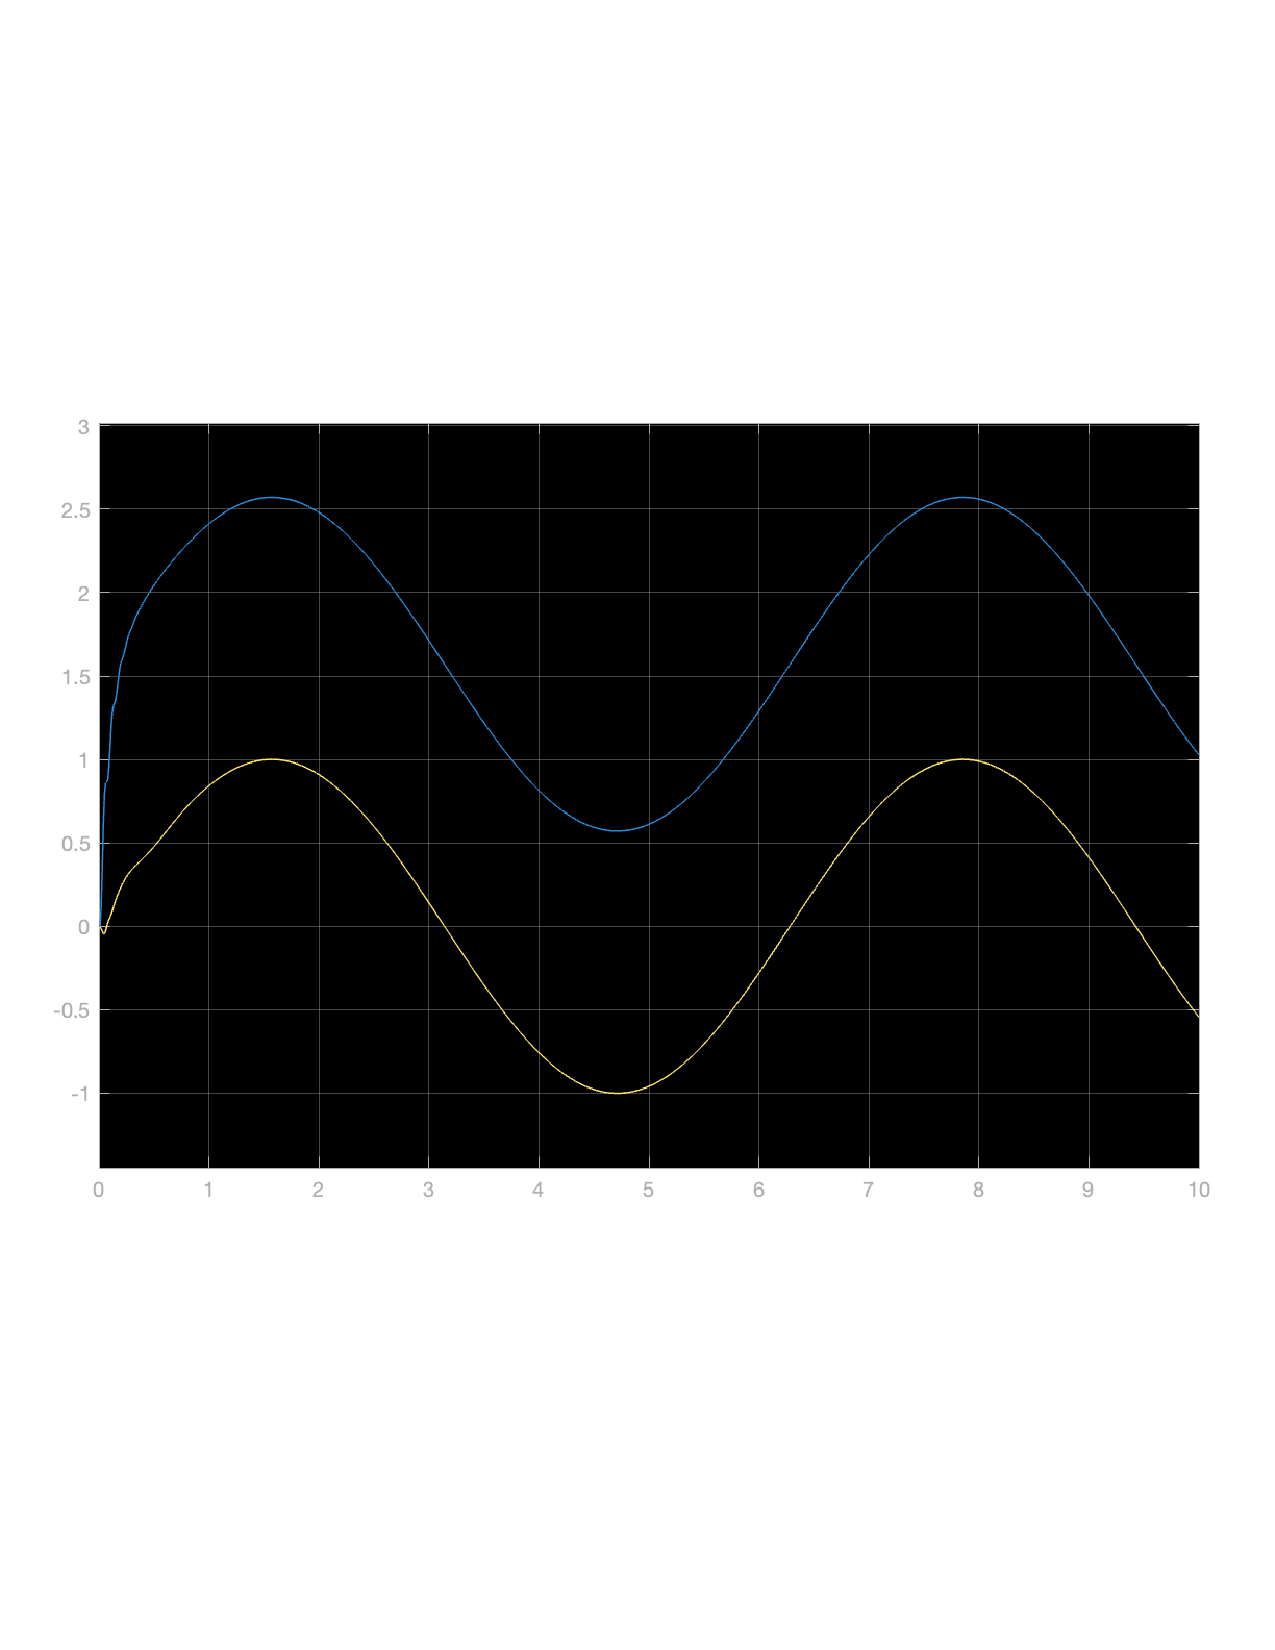
\includegraphics[width=0.8\textwidth]{figures/result_computed.pdf}
    \caption{Result Plot, error disappeared after 1 second}
    \label{fig:result_computed_plot}
\end{figure}



\newpage

\section{Explanation}
The first thing I need to mention is I found I calculated the $M$ and $V$ matrices wrong in the past simulations, so I fixed the problem and now robot dynamics runs normally.\\

\subsection{Passivity-based task-space controller}
For this part, it is important to understand the Jacobian matrix and simple forward kinematics for 2-dof joints. After that, everything goes simple.\\ 


\subsection{Computed torques controller}
For this part, an interesting thing I found is that even if I don't add the inverse dynamic block and modify the controller part, the result is still ok.\\

The inverse dynamic block is very simple to make, almost the same as the robot dynamic, you just need to change the input and output of the function.

\end{document}